\documentclass[10pt]{beamer}
\usepackage[utf8]{inputenc}
\usepackage{tikz}
\usetikzlibrary{shapes, arrows.meta, positioning}

\usepackage[absolute,overlay]{textpos}
\usepackage{graphicx}
\usepackage{listings}
\lstset{
  language=Python,
  basicstyle=\ttfamily\scriptsize,
  commentstyle=\color{gray},
  keywordstyle=\color{blue},
  stringstyle=\color{red},
  showstringspaces=false,
  numbers=left,
  numberstyle=\tiny,
  frame=single,
  breaklines=true,
}

\mode<presentation> {
\usetheme{boxes} % When headline is wanted use Dresden theme instead
\usecolortheme{seagull}
\logo{
\includegraphics[height=1.5cm]{ku_logo_dk}}
\setbeamertemplate{footline}[frame number]
% \setbeamertemplate{footline}{
%   \hspace{1em}
%   \hfill
%   \insertframenumber/\inserttotalframenumber
%   \vspace{1em}
%   \hspace{1em}
%   
\includegraphics[height=2cm]{ku_logo_dk}
%   \hspace{1em}
% }
\setbeamertemplate{navigation symbols}{}
\setbeamertemplate{itemize items}[square]
}


%----------------------------------------------------------------------------------------
%	TITLE PAGE
%----------------------------------------------------------------------------------------

\title[Kickstart-kursus] % bottom of every slide
  {Kickstart-kursus i programmering 23 dag 3\\ 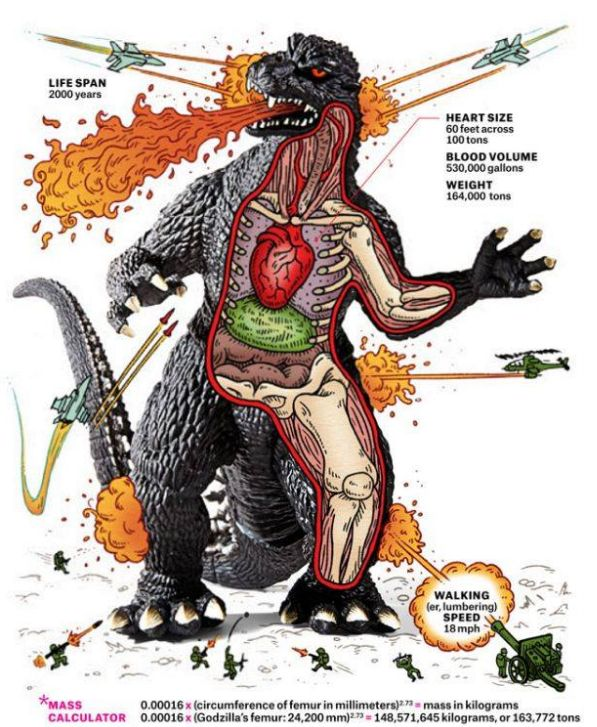
\includegraphics[height=5cm]{images/gozz}} % title page



\author{\footnotesize{Daniel Spikol} \\
          \footnotesize{\texttt{ds@di.ku.dk}}}

\institute {DIKU \\ Københavns Universitet}

\date[16. august 2023]{16 august 2023}

\begin{document}
\begin{frame}[plain]
\titlepage
\end{frame}
%%----------------------------------------------%%
\begin{frame}{Recap from Tuesday}
   	\begin{itemize}
	\item Python and Functions
	\item Animations
	\item Pair Programming
	\item Mouse and Key Input
	\end{itemize}
\end{frame}

%%----------------------------------------------%%

\begin{frame}{Wednesday IFOs}
  \begin{itemize}
  \item Variable Scoping
   \item Draw() function
  \item Conditionals
  \item Ideation
  \end{itemize}
\end{frame}

%%----------------------------------------------%%

\begin{frame}{Variable Scoping Py.Processing}
\begin{itemize}
\item The principles of variable scoping in Processing.py largely follow those
of Python but with some considerations given the environment of
Processing's draw loop and function setup.
\item Scoping in programming refers to the region or portion of the code where a variable or function is defined and can be accessed or modified. 
\item The concept of scoping is crucial for understanding variable lifetimes, visibility, and potential naming conflicts in your programs. It helps manage and organize data and functionality, enabling modular and maintainable code designs.
\end{itemize}
\end{frame}
%%----------------------------------------------%%

\begin{frame}[fragile]{Variable Scoping Py.Processing}{Global Variables }

\textbf{Global Variables}: Variables declared outside of any function
are global to the sketch. They can be accessed and modified from any
function, but if you want to modify them inside a function, you must declare them as \texttt{global} within that function.

\begin{lstlisting}
#global in action
x = 10

def changeX():
    global x
    x = 20
\end{lstlisting}	
\end{frame}


%%----------------------------------------------%%

\begin{frame}[fragile]{Variable Scoping Py.Processing}{Local Variables }
  
  \textbf{Local Variables}: Variables declared inside a function are
  local to that function. They cannot be accessed outside of the
  function, and their memory is reclaimed once the function execution is
  complete.
  \begin{lstlisting}
def showValue():
    y = 15
    print(y)  # This will print 15
    
showValue()
# print(y)  # This would be an error because y is not defined outside of the function.\end{lstlisting}	

\end{frame}

%%----------------------------------------------%%

\begin{frame}[fragile]{Variable Scoping Py.Processing}

\textbf{The setup() and draw() Functions}: In Processing.py,
\texttt{setup()} is called once at the beginning of the sketch, and
\texttt{draw()} is called repeatedly, producing frames. 
\begin{lstlisting}
x = 0

def setup():
    global x
    size(400, 400)
    x = width / 2  # Initializing x based on the canvas width
    
def draw():
    global x
    background(240)
    ellipse(x, height/2, 50, 50)
    x += 1
\end{lstlisting}

Variables declared in \texttt{setup()} are local to \texttt{setup()}. Still, often you want to declare global variables at the top level of your sketch and then initialise or modify them in \texttt{setup()}.

\end{frame}

%%----------------------------------------------%%
\begin{frame}{Conditionals in Computer Science}
\begin{itemize}
\item Conditionals in computer science refer to constructs that allow for decision-making in code. 
\item They determine the flow of execution based on whether a given condition is true or false. 
\item Depending on the outcome of the condition, different blocks of code will be executed.
\item Specifically, conditionals perform different computations or actions depending on whether a programmer-defined boolean condition evaluates to true or false.
\end{itemize}
\end{frame}

%%----------------------------------------------%%

\begin{frame}{Conditionals Conceptually}
\begin{itemize}
    \item \textbf{Basic Conditional (IF)}
    \textit{Concept}: If a specific condition is true, do something.
    \textit{Example}: ``If it's raining, take an umbrella.''
    \item \textbf{Alternative Path (ELSE)}
    \textit{Concept}: If the first condition isn't met, do something else instead.
    \textit{Example}: ``If it's raining, take an umbrella. Otherwise, wear sunglasses.''
    \item \textbf{Multiple Conditions (ELSE IF or ELIF)}
    \textit{Concept}: Check multiple conditions in sequence, and do the first thing that's true.
    \textit{Example}: ``If it's raining, take an umbrella. If it's sunny, wear sunglasses. Otherwise, just go outside as usual.''
    \item \textbf{Combining Conditions}
    \textit{Concept}: You can use logical operators (AND, OR, NOT) to combine conditions.
    \textit{Example}: ``If it's a weekend AND the weather is good, go hiking.''
\end{itemize}

\end{frame}

%%----------------------------------------------%%

\begin{frame}{UML Condition}
\begin{center}
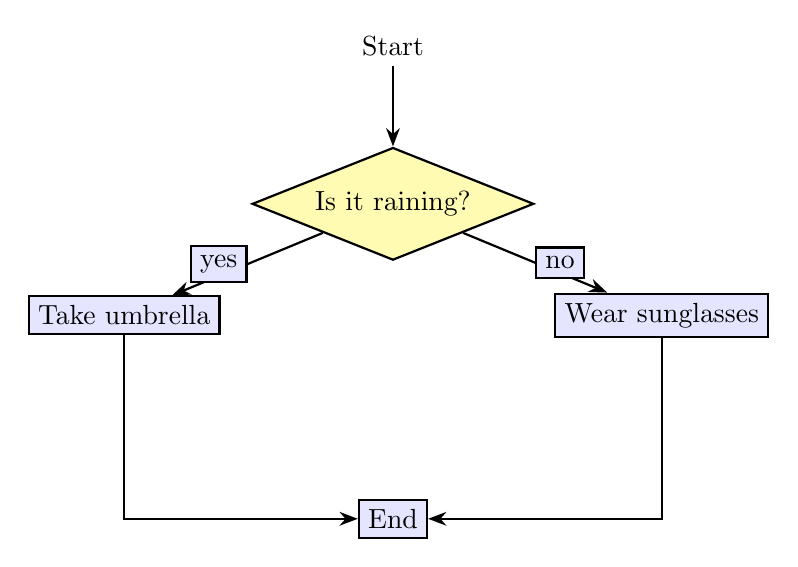
\begin{tikzpicture}[node distance=2cm, 
                    every node/.style={rectangle, draw, fill=blue!10},
                    thick,>=Stealth]

% Nodes
\node (start) [draw=none,fill=none] {Start};
\node (check) [below of=start, diamond, aspect=2.5, fill=yellow!30] {Is it raining?};
\node (umbrella) [below left of=check, xshift=-2cm] {Take umbrella};
\node (sunglasses) [below right of=check, xshift=2cm] {Wear sunglasses};
\node (end) [below of=check, yshift=-2cm] {End};

% Edges
\draw[->] (start) -- (check);
\draw[->] (check) -- node[left] {yes} (umbrella);
\draw[->] (check) -- node[right] {no} (sunglasses);
\draw[->] (umbrella) |- (end);
\draw[->] (sunglasses) |- (end);

\end{tikzpicture}
\end{center}

\end{frame}

%%----------------------------------------------%%
\begin{frame}{Cake Condition}
\begin{center}
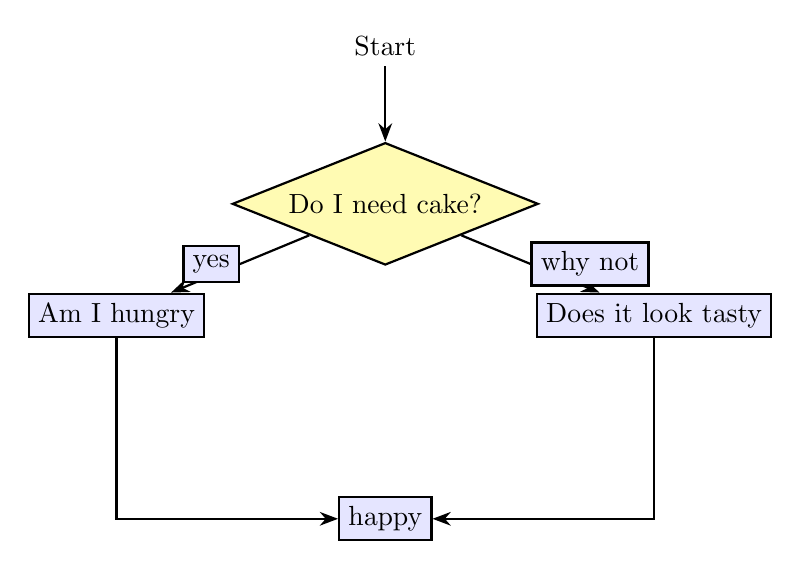
\begin{tikzpicture}[node distance=2cm, 
                    every node/.style={rectangle, draw, fill=blue!10},
                    thick,>=Stealth]

% Nodes
\node (start) [draw=none,fill=none] {Start};
\node (check) [below of=start, diamond, aspect=2.5, fill=yellow!30] {Do I need cake?};
\node (hunger) [below left of=check, xshift=-2cm] {Am I hungry};
\node (desire) [below right of=check, xshift=2cm] {Does it look tasty};
\node (happy) [below of=check, yshift=-2cm] {happy};

% Edges
\draw[->] (start) -- (check);
\draw[->] (check) -- node[left] {yes} (hunger);
\draw[->] (check) -- node[right] {why not} (desire);
\draw[->] (hunger) |- (happy);
\draw[->] (desire) |- (happy);

\end{tikzpicture}
\end{center}

\end{frame}

%%----------------------------------------------%%

\begin{frame}{Conditionals}
\begin{itemize}
\item \textbf{If Statement:} Executes a code block if a specified condition is true.
\item \textbf{Else Statement:} Used in conjunction with an if statement, it specifies a block of code to be executed if the condition in the if statement is false.
\item \textbf{Else If Statement:} Used to specify a new condition to test if the first condition is false.
\item \textbf{Switch or Case Statement:} Allows a variable to be tested for equality against a list of values.
\end{itemize}
\end{frame}

%%----------------------------------------------%%

\begin{frame}{Conditionals in Python}
Python supports the usual logical conditions from mathematics:
\begin{itemize}
\item Equals: \texttt{a == b}
\item Not Equals: \texttt{a != b}
\item Less than: \texttt{a < b}
\item Less than or equal to: \texttt{a <= b}
\item Greater than: \texttt{a > b}
\item Greater than or equal to: \texttt{a >= b}
\end{itemize}
\end{frame}

%%----------------------------------------------%%

\begin{frame}[fragile]{Conditionals in Python}
\texttt{if:}
\begin{lstlisting}
if x > 10:
    print("x is greater than 10")
\end{lstlisting}

\texttt{elif (else if):}
\begin{lstlisting}
if x > 10:
    print("x is greater than 10")
elif x == 10:
    print("x is 10")
\end{lstlisting}

\texttt{else:}
\begin{lstlisting}
if x > 10:
    print("x is greater than 10")
else:
    print("x is 10 or less")
\end{lstlisting}

You can also combine conditions using logical operators (\texttt{and, or, not}):
\begin{lstlisting}
if x > 10 and y < 5:
    print("x is greater than 10 and y is less than 5")
\end{lstlisting}
\end{frame}

%%----------------------------------------------%%
\begin{frame}[fragile]{Conditionals in Py.Processing}
For instance, to animate a circle moving across the screen and to make it wrap around when it reaches the edge:
\begin{lstlisting}
x_pos = 0

def setup():
    size(400, 400)

def draw():
    global x_pos
    background(240)
    ellipse(x_pos, height/2, 50, 50)
    x_pos += 2

    # Conditional to check if the circle is out of bounds
    if x_pos > width:
        x_pos = 0
\end{lstlisting}

In the code above, the conditional if \texttt{if x\_pos > width:} checks if the circle has moved outside the canvas. If true, it resets its position.
\end{frame}


%%----------------------------------------------%%
\begin{frame}{IDEAL Problem Solving}
\begin{center}
    	 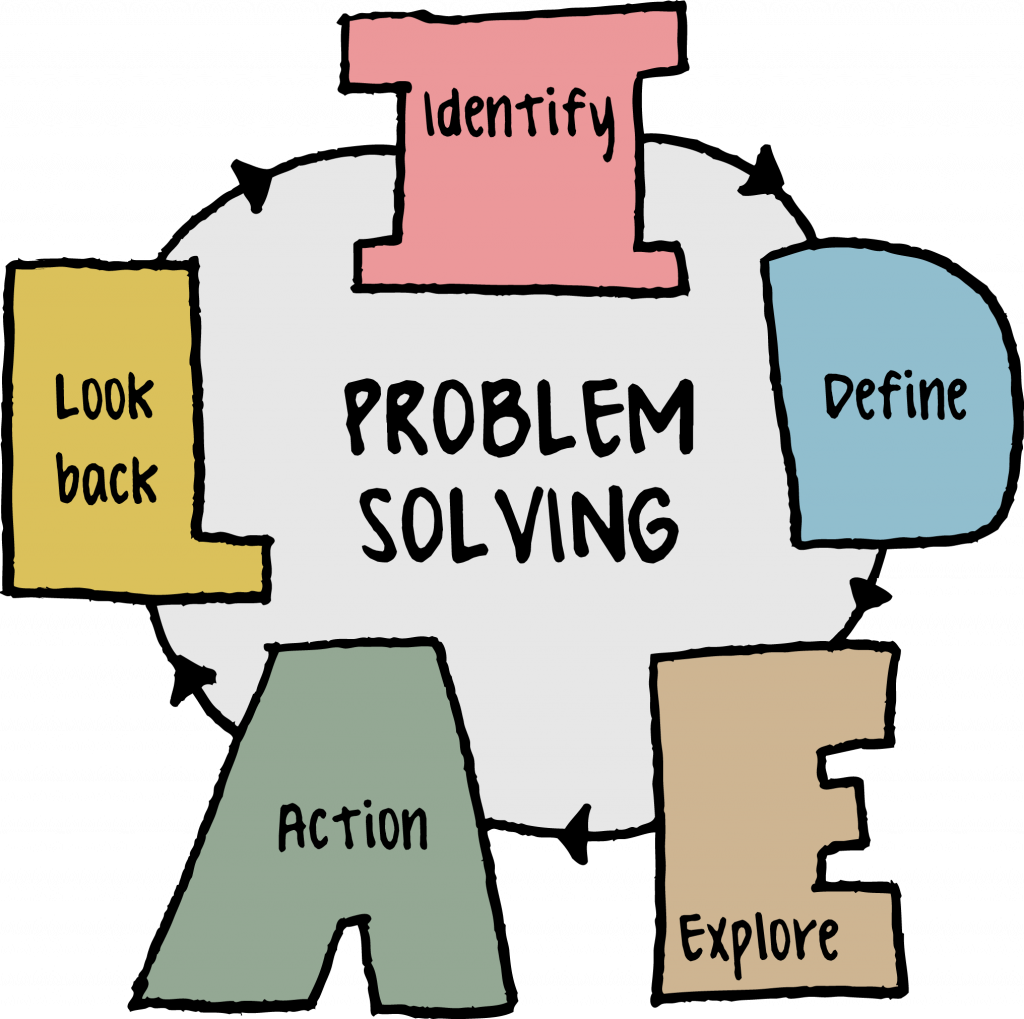
\includegraphics[height=7cm]{images/ideal_ps}
\end{center}
\end{frame}

%%----------------------------------------------%%
%%----------------------------------------------%%
\begin{frame}{Today' Recap}
   	\begin{itemize}
	\item Conditionals
	\item Better Animations
	\item Pair Programming
	\item Ideas for Projects
	\end{itemize}
\end{frame}

%%----------------------------------------------%%

\begin{frame}{Tomorrow}
   	\begin{itemize}
	\item Finite State Machines
	\item Project Work
	\item Coding
	\end{itemize}
\end{frame}
%%----------------------------------------------%%
%%----------------------------------------------%%
%%----------------------------------------------%%
\end{document}